\documentclass{scrartcl}
\usepackage[a4paper,left=1in,right=1in,top=1.2in,bottom=1in]{geometry}
\usepackage{siunitx}
\usepackage{graphicx}
\usepackage{mathtools}
\setkomafont{disposition}{\normalfont\bfseries}
\newcommand*\diff{\mathop{}\!\mathrm{d}}
\newcommand*\Diff[1]{\mathop{}\!\mathrm{d^#1}}
\newcommand*\colvec[3][]{
    \begin{pmatrix}\ifx\relax#1\relax\else#1\\\fi#2\\#3\end{pmatrix}
}

%title
\title{Exercise 05:\\Rescorla-Wagner rule}
\subtitle{Theoretical Neuroscience II}
\author{Johannes G\"atjen \and Lorena Morton}

%use these for structure/overview
\newcommand\Question{%
  \textbf{Question:}%
}
\newcommand\Answer{%
  \textbf{Answer:}%
}
\renewcommand{\arraystretch}{1.2}


\begin{document}
\maketitle

\section{Two independent stimuli}

We consider two independent stimuli, $A$ and $B$, that are present according to the following probability table:\\
\begin{tabular}{c | c c | c}
& $A$ & $\neg A$ & \\  [3pt] \hline
$B$ & $\frac{1}{15}$ & $\frac{2}{15}$ & $\frac{1}{5}$ \\ [3pt]
$\neg B$ & $\frac{2}{15}$ & $\frac{8}{15}$ & $\frac{4}{5}$\\ [3pt] \hline
& $\frac{1}{3}$ & $\frac{2}{3}$ & 1 \\ [3pt]
\end{tabular}\\

From the probability table we can compute the expected stimulus vector $\langle \mathbf{u} \rangle$, the correlation matrix $\mathbf{Q}$ and its inverse:
\begin{align*}
\langle \mathbf{u} \rangle = \colvec{p_A}{p_B} = \colvec{\frac{1}{3}}{\frac{1}{5}}\\
\mathbf{Q} = \left( \begin{array}{cc}
\langle u_1^2 \rangle & \langle u_1u_2 \rangle \\
\langle u_1u_2 \rangle & \langle u_2^2 \rangle \end{array} \right) = \left( \begin{array}{cc}
\frac{1}{3} & \frac{1}{15} \\
\frac{1}{15} & \frac{1}{5} \end{array} \right) \\
\mathbf{Q}^{-1} = \left( \begin{array}{cc}
\frac{45}{14} & -\frac{15}{14} \\
-\frac{15}{14} & \frac{225}{42} \end{array} \right) 
\end{align*}

\section{Full, partial and inhibitory conditioning}

When we get a reward $r = 1$ whenever $A$ is present we get the following joint expectation of stimulus and reward $\langle r \mathbf{u}\rangle$, conditional expectation of reward, given stimulus $\langle r \mid \mathbf{u}\rangle$ and the asymptotic weights for the Rescorla-Wagner rule $\mathbf{w}_{ss}$.
\begin{align*}
\langle r \mathbf{u}\rangle = \colvec{\frac{1}{3}}{\frac{1}{15}} \qquad
\langle r \mid \mathbf{u}\rangle = \colvec{1}{\frac{1}{3}} \qquad
\mathbf{w}_{ss} = \mathbf{Q}^{-1} \cdot \langle r \mathbf{u}\rangle = \colvec{1}{0}
\end{align*}
The conditional expectation of reward, given stimulus $\langle r \mid \mathbf{u}\rangle$ simply tells us how much certain stimuli occur together with rewards. The specific reward expectation on the other hand tells us which stimulus is responsible for the rewards. One can say that $\langle r \mid \mathbf{u}\rangle$ gives us a purely descriptive value, whereas $\mathbf{w}_{ss}$ tells us something about the (presumed) causality of the world.

Figure \ref{one} shows the development according to the Rescorla-Wagner rule with the probabilities and rewards as specified above with a learning rate of $\epsilon = 0.05$. Figure \ref{two} shows development of partial conditioning and Figure \ref{three} shows inhibitory conditioning.

\begin{figure}
\centering
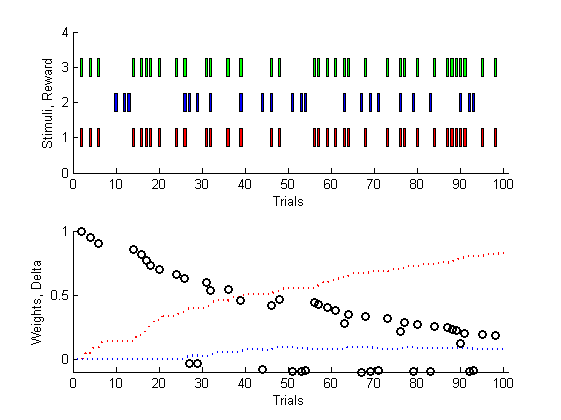
\includegraphics[trim = {0.8cm 0 0.5cm 0.2cm}, width=0.8\textwidth, clip]{../pics/one}
\caption{The first 100 trials for full conditioning. Top: Red: occurrences of stimulus $A$. Blue: occurrences of stimulus $B$. Green: occurrences of rewards ($r = 1$). Bottom: Red dotted line: Specific reward expectation for $A$. Blue dotted line: Specific reward expectation for $B$. Black circles: Prediction error $\delta$. Specific reward expectations after 1000 trials: $(1.00, 0.00)^T$.
Initially, the prediction errors are large, and the reward expectation is split between $A$ and $B$ evenly when they occur together. Then when $B$ occurs alone there is a small expectation of reward, but because there is no reward the prediction error is negative and the reward expectation for $B$ is decreased again. After enough trials the reward expectations have been learned correctly and the prediction errors are (almost) zero.}
\label{one}
\end{figure}

\begin{figure}
\centering
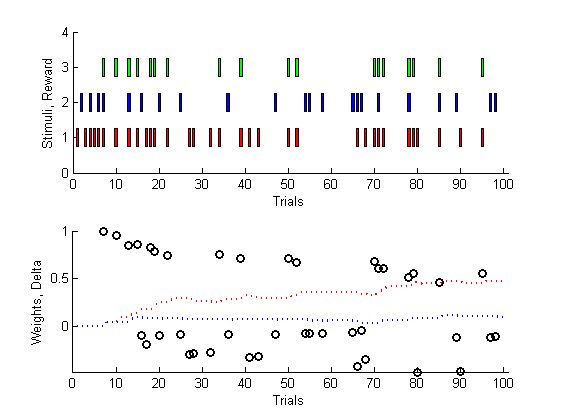
\includegraphics[trim = {0.8cm 0 0.5cm 0.2cm}, width=0.8\textwidth, clip]{../pics/two}
\caption{The first 100 trials for partial conditioning. Stimulus $A$ is rewarded with probability $0.5$. See Figure \ref{one} for plot details. Specific reward expectations after 1000 trials: $(0.53, 0.07)^T$.}
\label{two}
\end{figure}

\begin{figure}
\centering
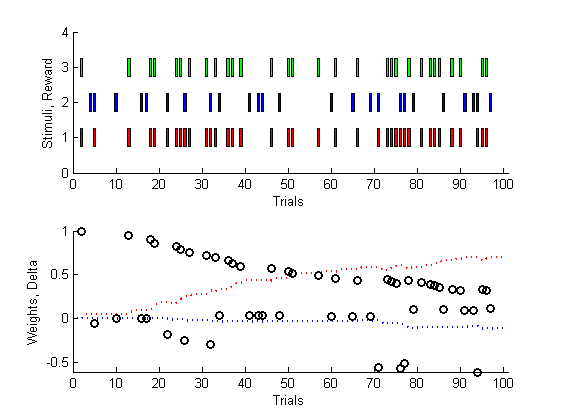
\includegraphics[trim = {0.8cm 0 0.5cm 0.2cm}, width=0.8\textwidth, clip]{../pics/three}
\caption{The first 100 trials for inhibitory conditioning. Stimulus $A$ is rewarded with probability $1$, but only if $B$ is absent. See Figure \ref{one} for plot details. Specific reward expectations after 1000 trials: $(0.86, -0.24)^T$. Stimulus $A$ is a predictor for reward, but stimulus $B$ prevents any rewards. Because there is no distinction between types of reward (only absence/presence/magnitude) the withdrawal of an expected reward is simply a negative reward (punishment) and is here associated with $B$.}
\label{three}
\end{figure}


\end{document}